\documentclass[a4paper,12pt]{article}
\usepackage{graphicx} 
\usepackage{amsmath} 
\usepackage{amssymb} 
\usepackage{geometry} 
\usepackage{fancyhdr} % for headers and footers
\usepackage{caption} % for customizing captions
\usepackage{subcaption}
\usepackage{setspace} 
\usepackage[bottom]{footmisc}
\usepackage{adjustbox}
\usepackage{placeins}
\usepackage{float}
\usepackage[nopatch=item]{microtype}
\usepackage{enumitem} % for customizing lists
\usepackage[backend=biber]{biblatex} % for bibliography
\usepackage[colorlinks,linkcolor=blue,citecolor=blue,urlcolor=blue]{hyperref}
\addbibresource{Sci. Data_01.bib} % specify your bibliography file

\setlength{\parindent}{1.27cm} % Indent first line of each paragraph by 1.27 cm (0.5 inches)

\geometry{margin=1in}
\setlength{\parindent}{0pt}
\setlength{\parskip}{6pt}
\doublespacing

 
\pagestyle{fancy}
\fancyhf{}
\fancyhead[L]{\leftmark}
\fancyfoot[C]{\thepage}

\begin{document}


\section*{Introduction}
Fourier transform is the most widely used tools in applied mathematics
to analyze signals. The essence of the Fourier transform of a waveform is to decompose
or separate the waveform into a sum of sinusoids of different frequencies.
If these sinusoids sum to the original waveform, then we have determined
the Fourier transform of the waveform.
Mathematically speaking, is it possible to write this relation as:
$$
\mathcal{F}(f) = \int_{-\infty}^{+\infty} s(t) e^{i2\pi f t} dt,
$$
where g(t) is the waveform to be decomposed into a sum of sinusoids
and G(f) is the Fourier transform of g(t).
%aggiungere perchè errori vanno come la radice 
As an example, consider the
pulse waveform (a) and its Fourier transform (b) shown the following figures.
\begin{figure}[H]
    \centering
    % First row with two images
    \begin{minipage}[b]{0.40\linewidth} % 45% of line width for the first image
        \centering
        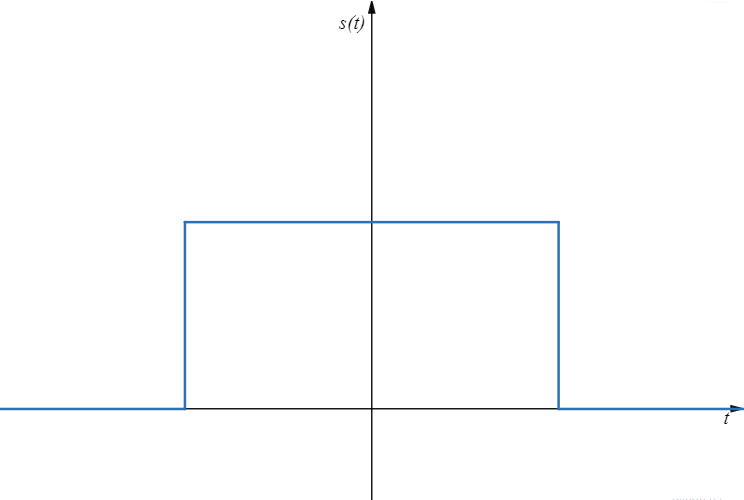
\includegraphics[width=\linewidth]{pulse.png}
        \caption{pulse waveform}
    \end{minipage}
    \hspace{0.05\linewidth} % Small horizontal space between images
    \begin{minipage}[b]{0.40\linewidth} % 45% of line width for the second image
        \centering
        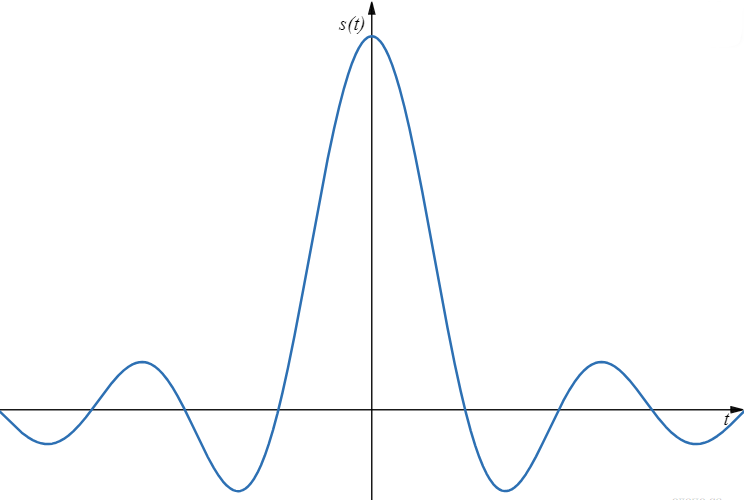
\includegraphics[width=\linewidth]{f.t_pulse.png}
        \caption{Fourier transform }
    \end{minipage}
\end{figure}
The purpose of this experiment is to use the Fourier transform to analyze a 
signal affected by noise and check if the noise is "white noise" and if the 
standard deviation of the mean decreases as the square root of the number of 
acquisitions.



\section{Materials and Methods}
\subsection{Equipment And Tools}
\begin{itemize}
    \item Digital storage oscilloscope (Siglent - SDS5034X)
    \item Waveform generator (Siglent - SDG6022X)
    \item Two BNC-to-BNC cables
    \item USB flash drive
\end{itemize}

\subsection{Experimental Procedure}
We started by connecting the digital oscilloscope to the waveform generator 
using BNC-to-BNC cables. Then, we proceeded to generate a sinusoidal signal 
with a frequency of 1 kHz and an amplitude of 2 Vpp, along with a noise signal, 
using the waveform generator.
Next, using a function of the digital oscilloscope, we were able to add the two signals.
The resulting waveform can be seen in the following figures. 

\begin{figure}[H]
    \centering
    % First row with two images
    \begin{minipage}[b]{0.45\linewidth} % 45% of line width for the first image
        \centering
        \label{fig:sin}
        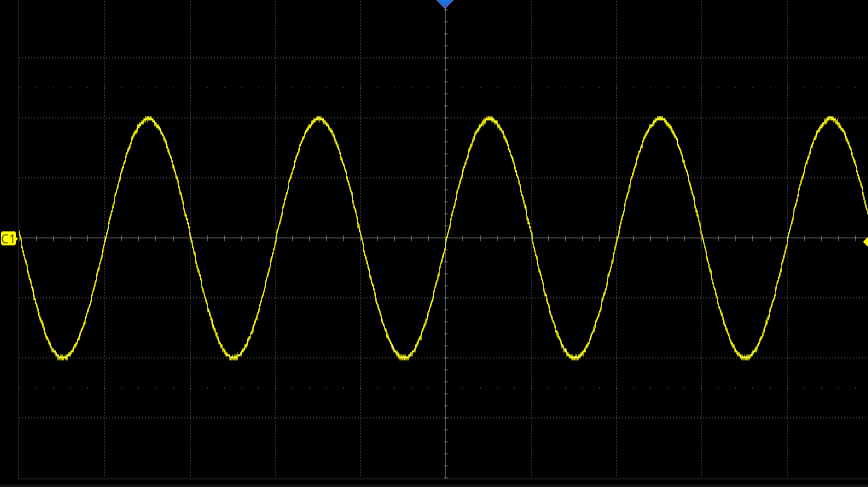
\includegraphics[width=\linewidth]{sin.png}
        \caption{Sinusoidal signal}
    \end{minipage}
    \hspace{0.05\linewidth} % Small horizontal space between images
    \begin{minipage}[b]{0.45\linewidth} % 45% of line width for the second image
        \centering
        \label{fig:noise}
        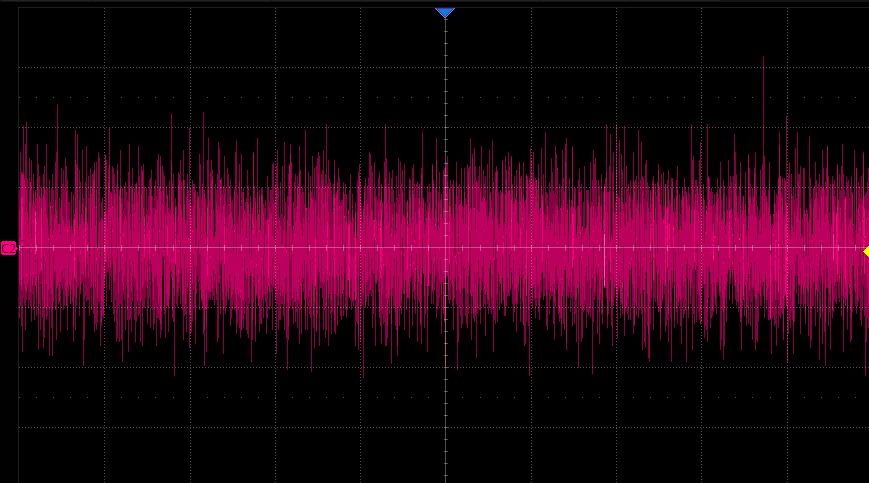
\includegraphics[width=\linewidth]{noise.png}
        \caption{Noise signal}
    \end{minipage}
    
    % Second row with centered image
    \vspace{0.5cm} % Vertical space between rows
    \begin{minipage}[b]{0.45\linewidth} % 60% of line width for the third image
        \centering
        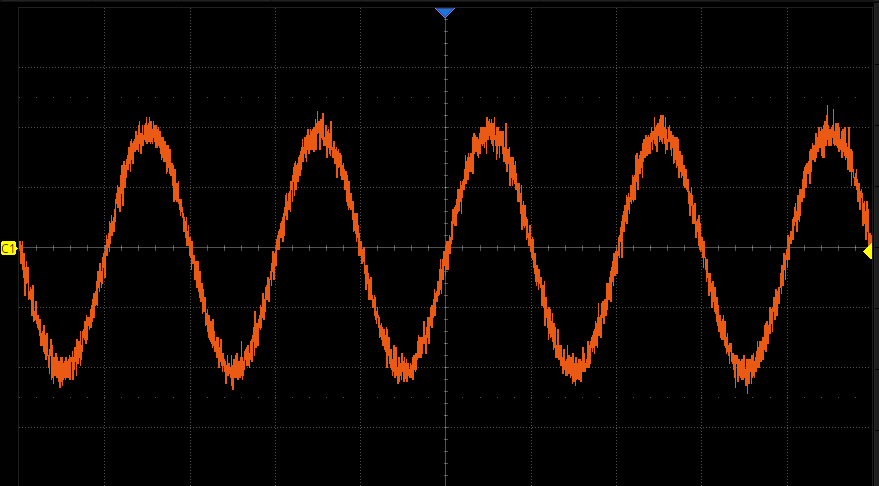
\includegraphics[width=\linewidth]{noise_signal.png}
        \label{fig:sin+noise_signal}
        \caption{Resulting signal from the addition of the two signals} 
    \end{minipage}
    
\end{figure}
Finally, we proceeded to acquire the data from the oscilloscope and saved it to a USB flash drive.
To acquire the data from the oscilloscope, we followed the steps below:
\begin{itemize}
    \item press the save/recall button, to open the file acquisitions menu
    \item select the the file extension, in our case .csv
    \item select our USB flash drive from the acquisition menu
    \item press on the touch screen the save as window
    \item select the file name and press the save button
\end{itemize}
All the data acquired was analyzed using Julia programming language 
% \cite{}. mettere su e aggingere la citazione al sito di julia https://julialang.org/
 







\newpage
%parte di mikk






\section{Results}
\subsection{Part 1}
\subsubsection{Original signal and its Fourier transform}
\par Once collected the data, we procede with the visualization of the data 
in graphical form. The following Fig (\ref{plot:raw_signal_and_noise}) 
shows the signal saved from the oscilloscope without any data processing. 
We can compare this plot with the image acquired directly from the oscilloscope
in Fig (\ref{fig:sin+noise_signal}) and check for their similarity.
\begin{figure}[H]
    \centering
    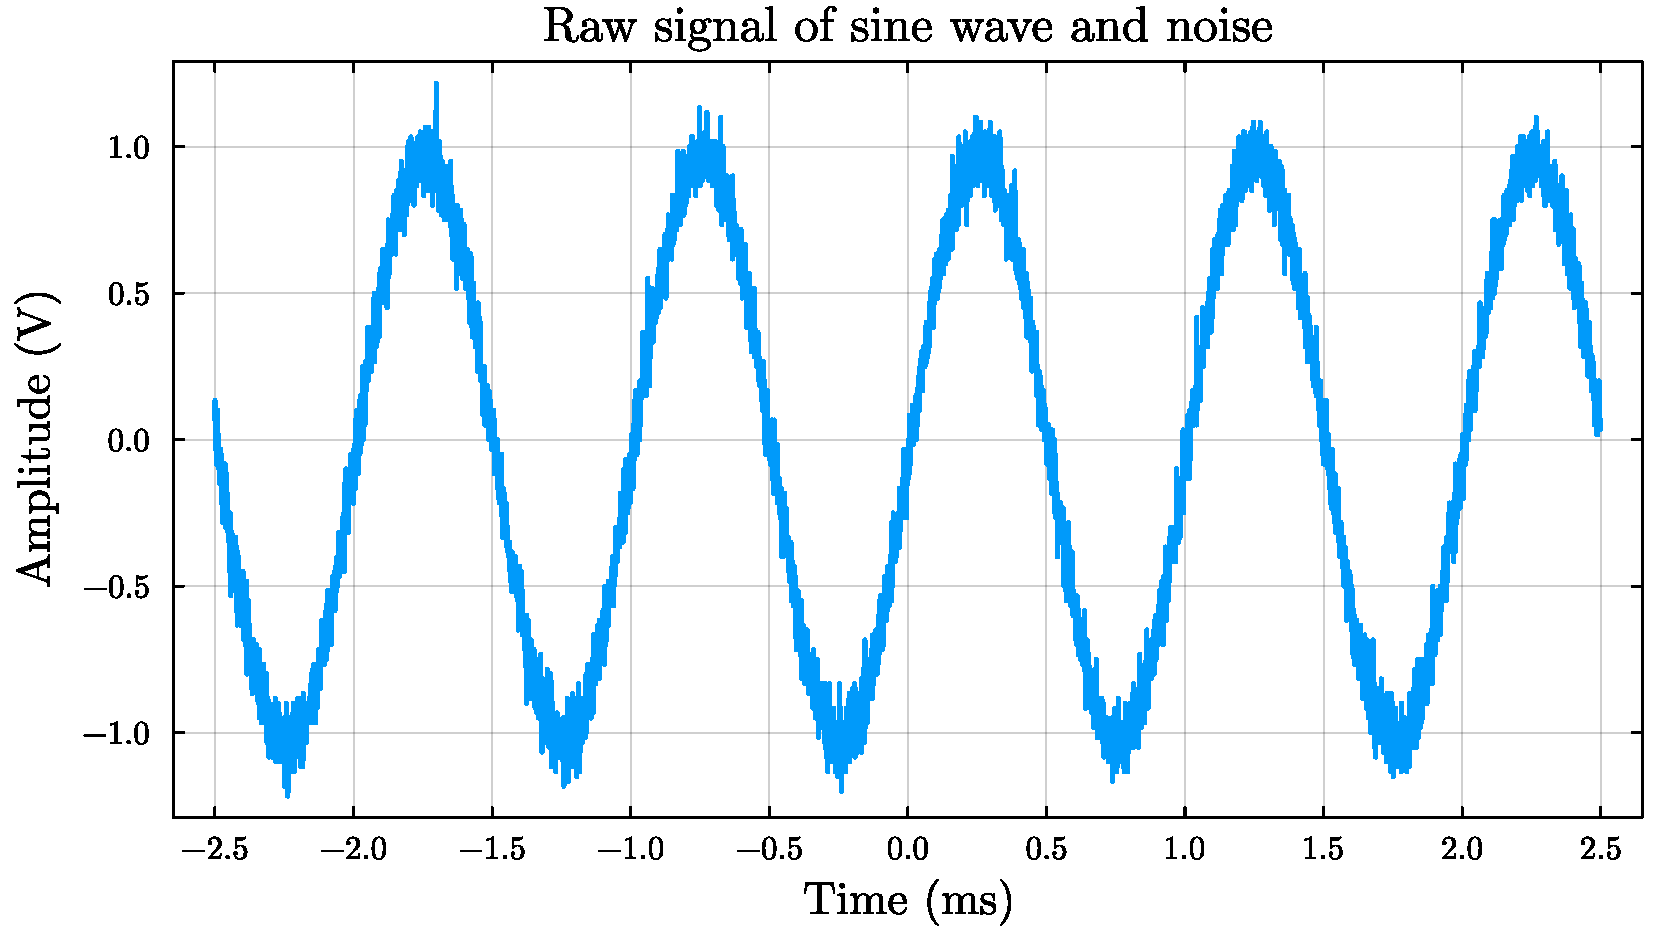
\includegraphics[width=0.9\textwidth]{signal01.pdf}
    \caption{One of our saved signal, composed of one sine wave and some noise.}
    \label{plot:raw_signal_and_noise}
\end{figure}
\begin{figure}[H]
    \centering
    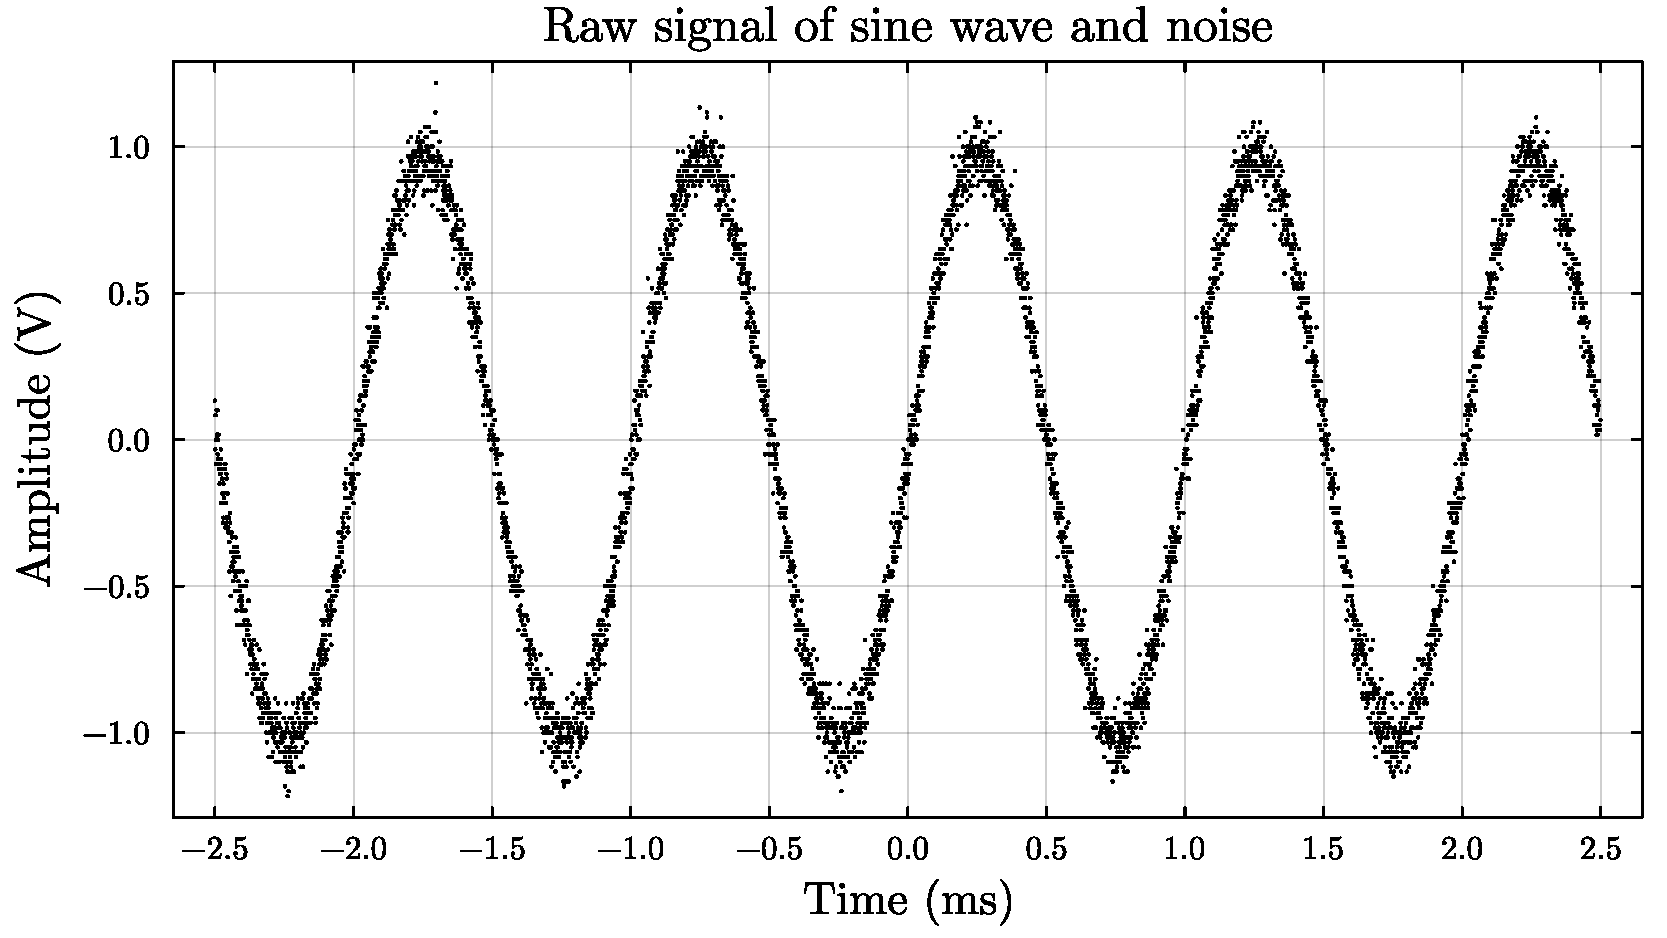
\includegraphics[width=0.9\textwidth]{signal01_scatter.pdf}
    \caption{One of our saved signal, composed of one sine wave and some noise.}
    \label{plot:raw_signal_and_noise_scatter}
\end{figure}

\par As our second step, we compute the Fourier transform of the previous signal, 
without using any windowing function. To do so, we take advantage of the library
"FFTW" of the julia programming language, this library implements both the
complex and real fourier transform, among with the inverse fourier transform 
and many other methods. For this experiment we will use the complex fourier transform.

\par After the transformation, we obtain an array of complex values. We will consider the
modulus of these numbers (which is the amplitude of the given frequency). Furthermore, 
we must say that the transform has non-zero values both in the positive and in the 
negative frequency axis. Our signal is of course made from real world data 
(in other words, real numbers), hence we can say that the final transformation will 
be an even function and the data on the negative side of the frequency axis will be 
a reflection of the data on the positive side of the same axis.

\par If we plot the values on the positive side only, we obtain the graph shown in 
Fig (\ref{plot:Fourier_signal}).
\begin{figure}[H]
    \centering
    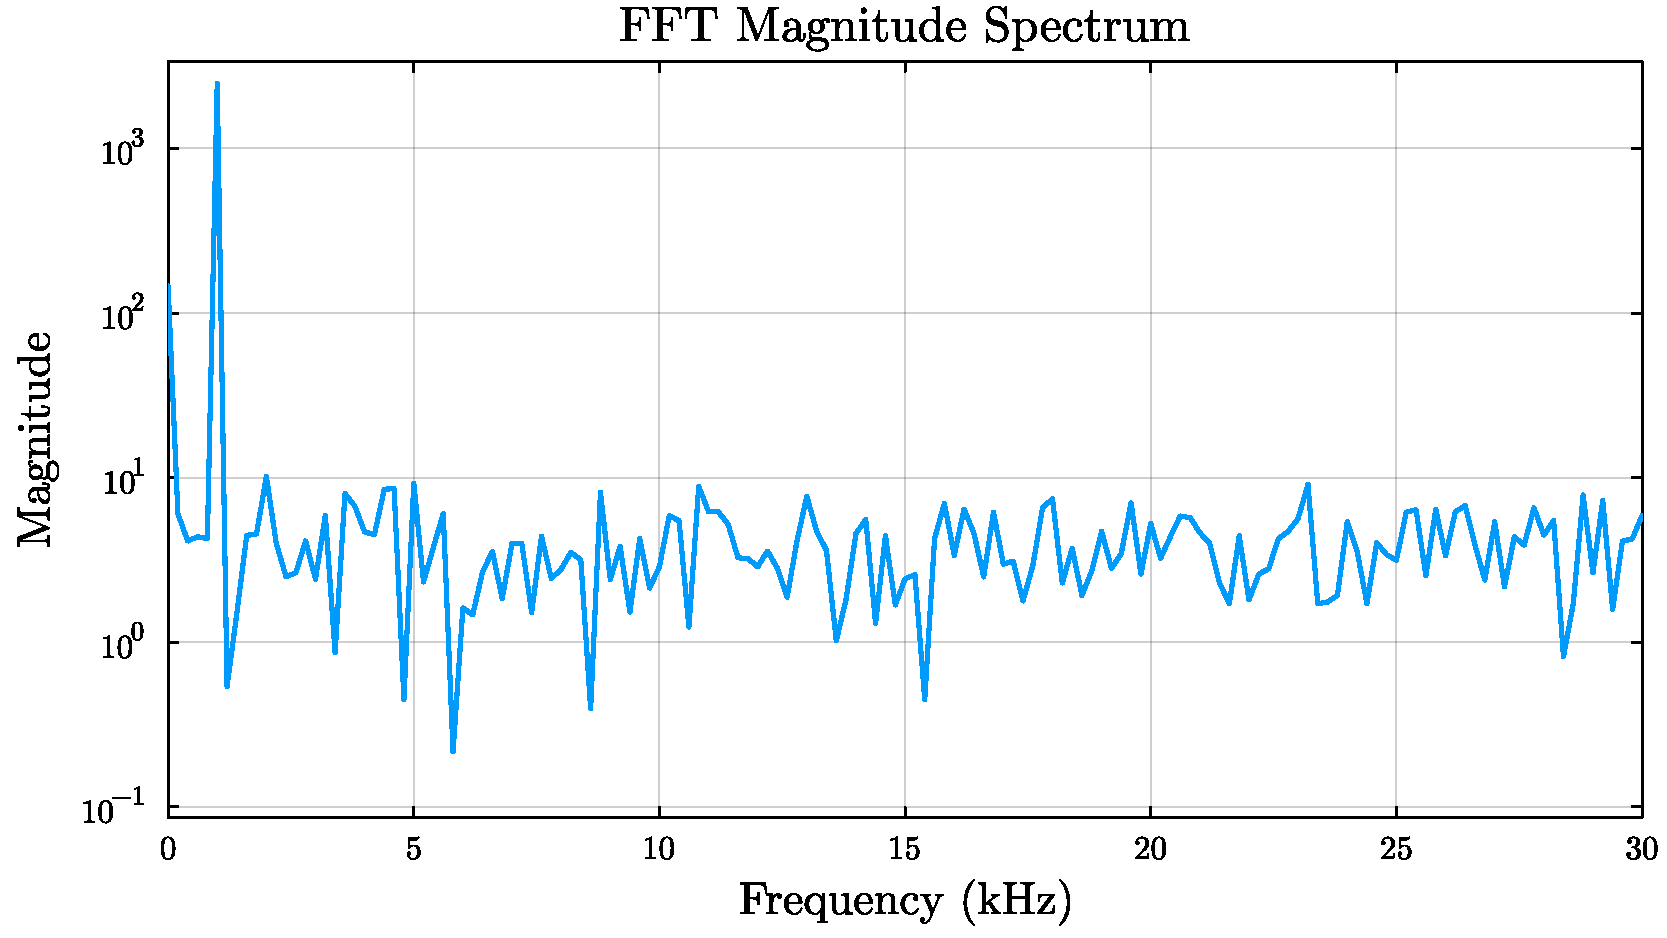
\includegraphics[width=0.9\textwidth]{fft01.pdf}
    \caption{Fast Fourier Transform of the signal}
    \label{plot:Fourier_signal}
\end{figure}
\begin{figure}[H]
    \centering
    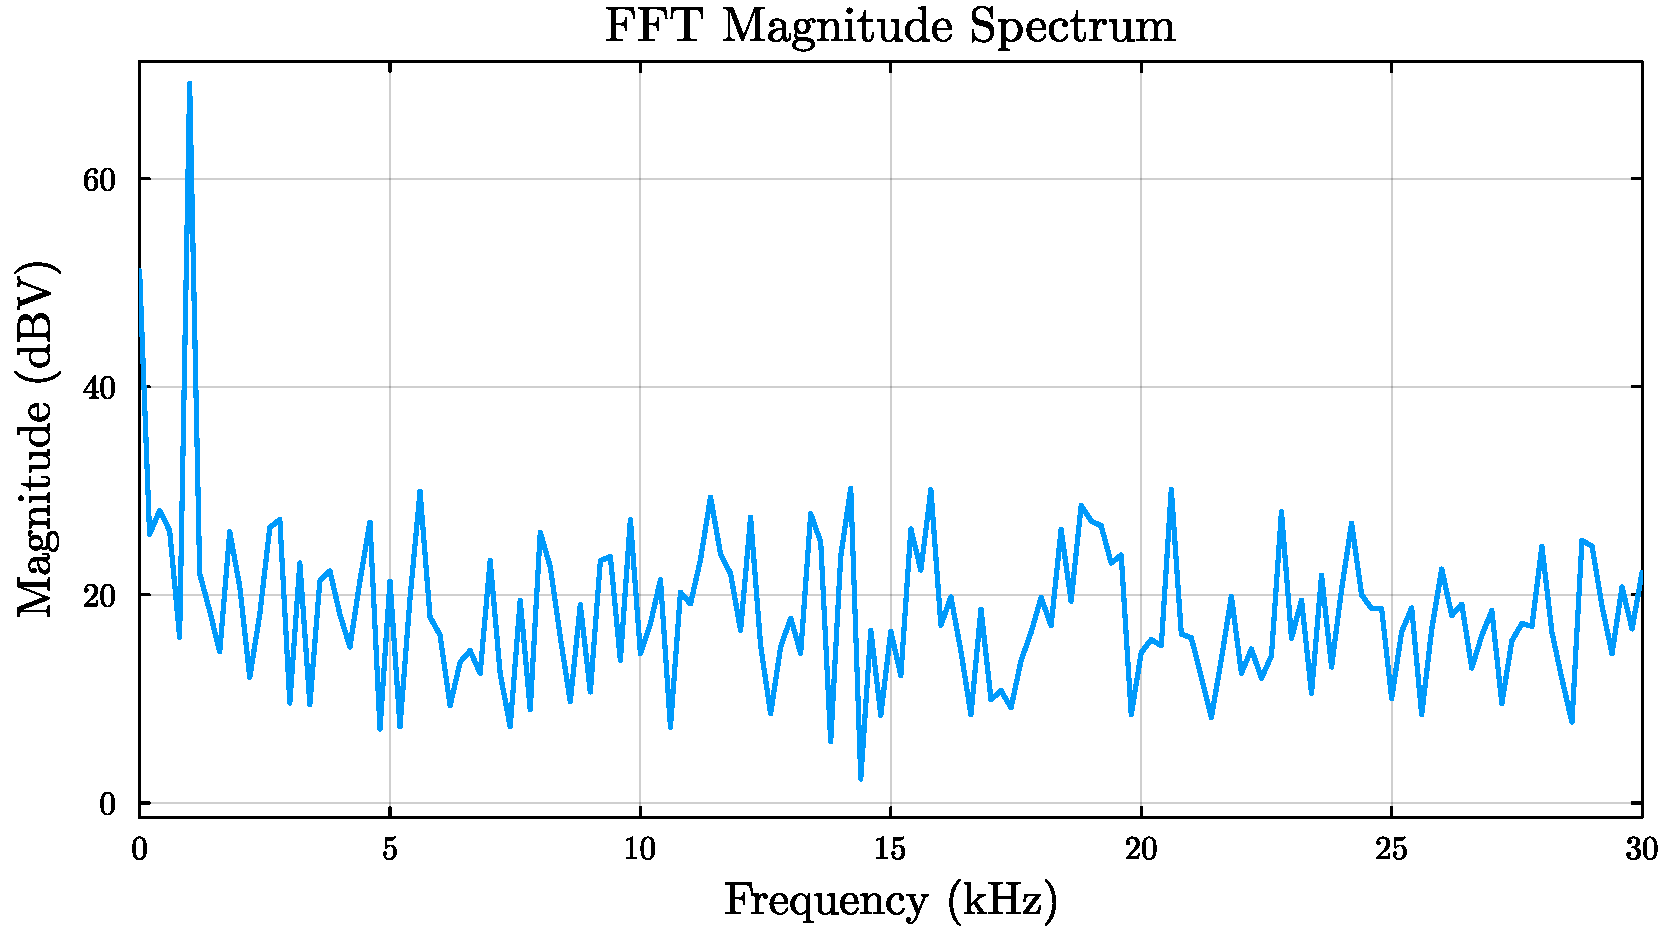
\includegraphics[width=0.9\textwidth]{fft01_dBV.pdf}
    \caption{Fast Fourier Transform of the signal in dBV}
    \label{plot:Fourier_signal_dBV}
\end{figure}

\par The plot in Fig (\ref{plot:Fourier_signal_dBV}) shows the Fourier transform in dBV.


\subsubsection{Peak cutoff and inverse Fourier transform }
\par We can now proceed in the selection of the frequencies which correspond to 
the noise. This step is equivalent to a peak removal, since we know that the signal 
which we are studying is a single sine wave. In practice, we modify the value of 
the Fourier transform in the position of the peak. We set this value to the mean 
of the transform in a big enought range (we use the interval $I$ from $1166$ to $4500$ Hz). 
We must remember to keep the transformation an even function, so we also modify the 
value of the transform for the negative frequency to the same value. In formulas, 
we impose 
\[
\begin{cases}
    \mathcal{F}(1000\, Hz) = \left\lang \mathcal{F}(f) \right\rang_I \\
    \mathcal{F}(-1000\, Hz) = \mathcal{F}(1000\, Hz)
\end{cases}.
\]

\par We can now evaluate the inverse transform in order to reconstruct the original noise.
We have a plot for the reconstructed noise in Fig (\ref{plot:Only_noise}).
\begin{figure}[H]
    \centering
    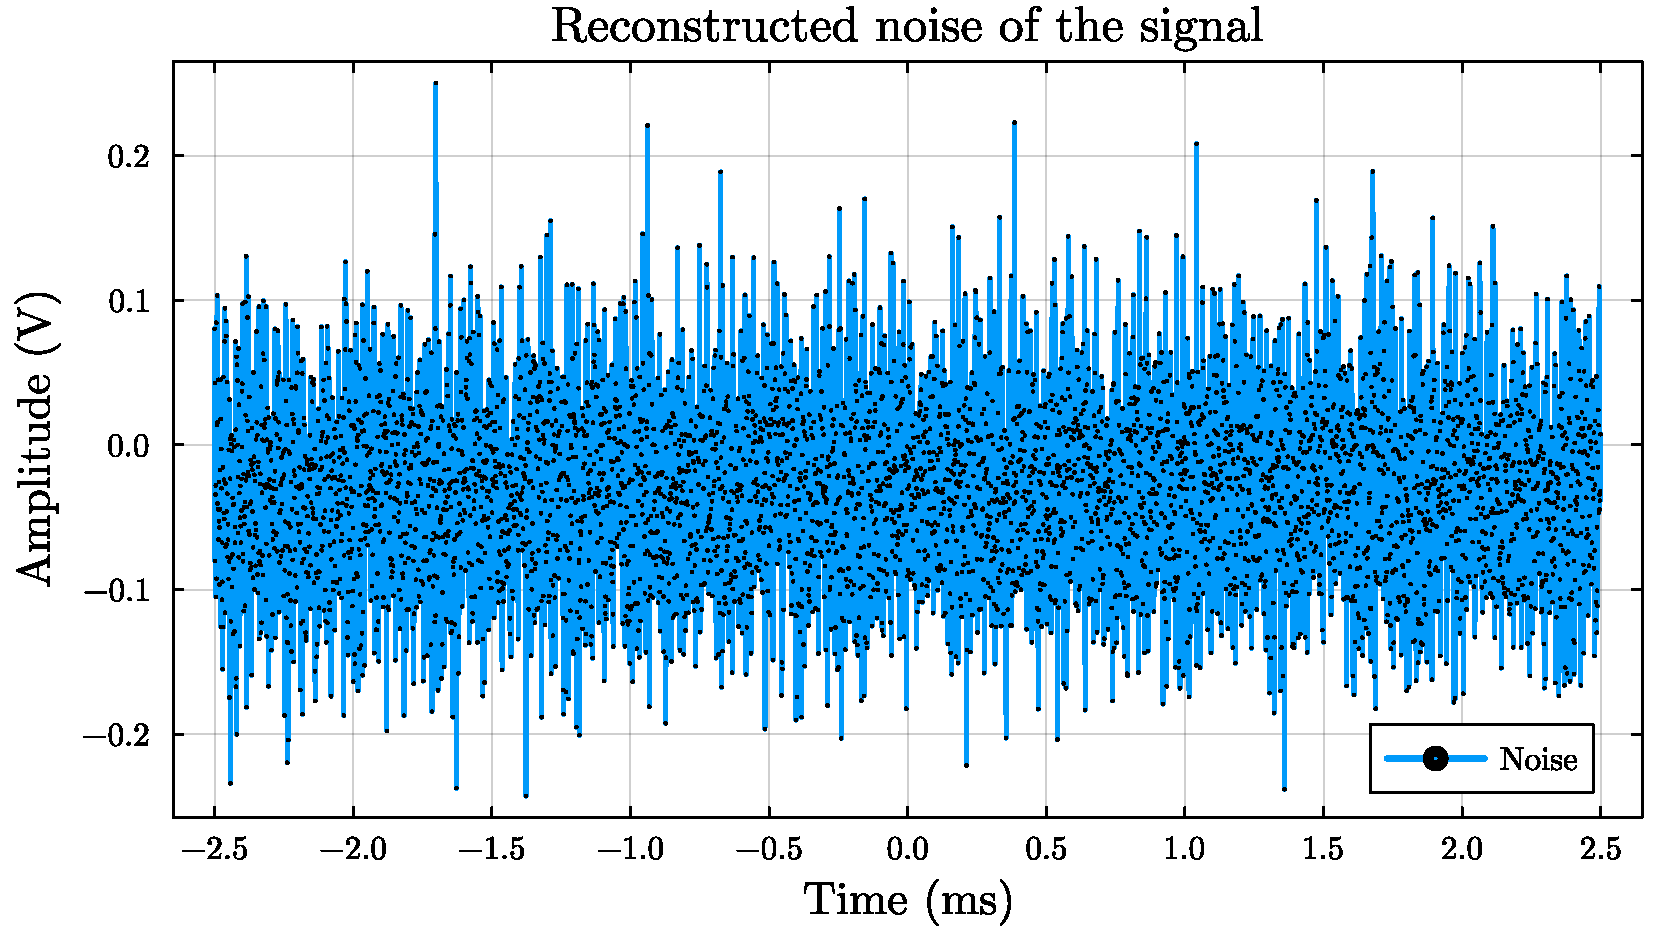
\includegraphics[width=0.9\textwidth]{signal01_only_noise.pdf}
    \caption{Reconstructed noise obtained from the inverse Fourier transform}
    \label{plot:Only_noise}
\end{figure}
\begin{figure}[H]
    \centering
    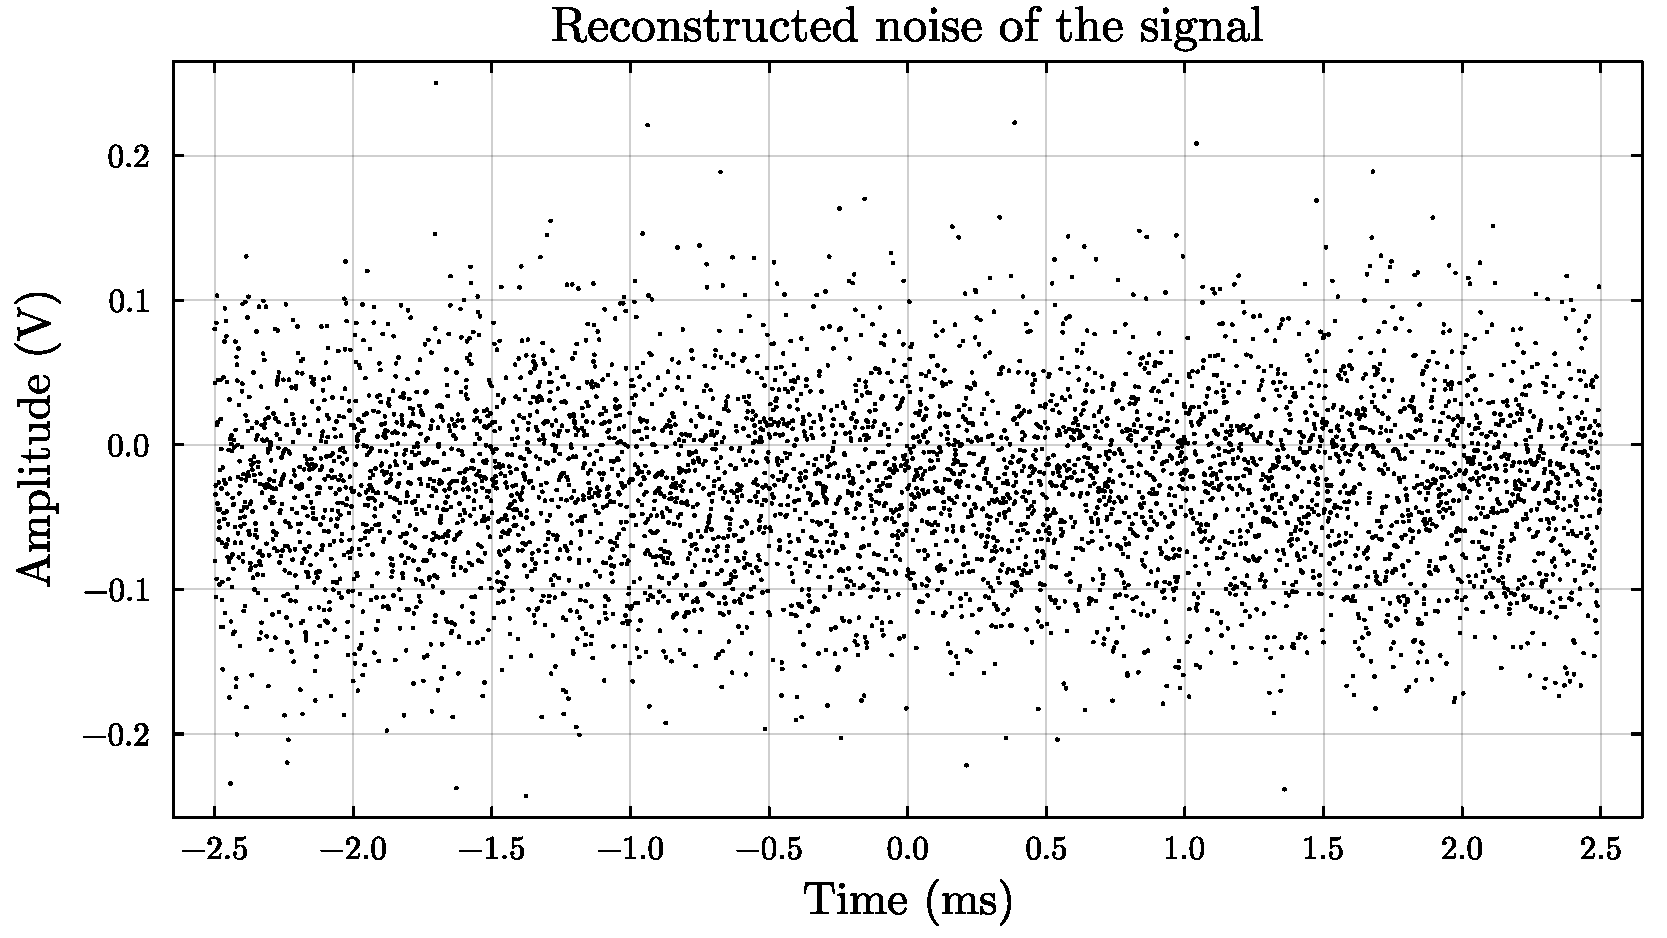
\includegraphics[width=0.9\textwidth]{signal01_only_noise_scatter.pdf}
    \caption{Reconstructed noise obtained from the inverse Fourier transform}
    \label{plot:Only_noise_scatter}
\end{figure}


\subsubsection{Statistical analysis of the reconstructed noise}
\par From the data obtained from the previos section, we can conduct 
a brief statistical analysis. The main purpose of this section is to 
check whether the noise obtained can be classified as white noise, that is 
noise that follows a normal distribution (also called Gaussian distribution).

\par We begin by calculating the mean ($\mu$) and the standard deviation 
($\sigma$) of the data, obtaining $\mu = -0.02925 \, mV$ and $\sigma = 0.06231 mV$.
As expected, the noise has a mean value very close to zero and the error is 
bigger than the mean, which means that the zero is inside the confidence 
range of $68\%$.  

\par We will now use the chi squared test to check how well the normal 
distribution fits our data. The Fig (\ref{plot:Hist_Gauss}) lets us see the expected 
values for this distribution in overlay with the normalized histogram 
of the data from the noise.
\begin{figure}[H]
    \centering
    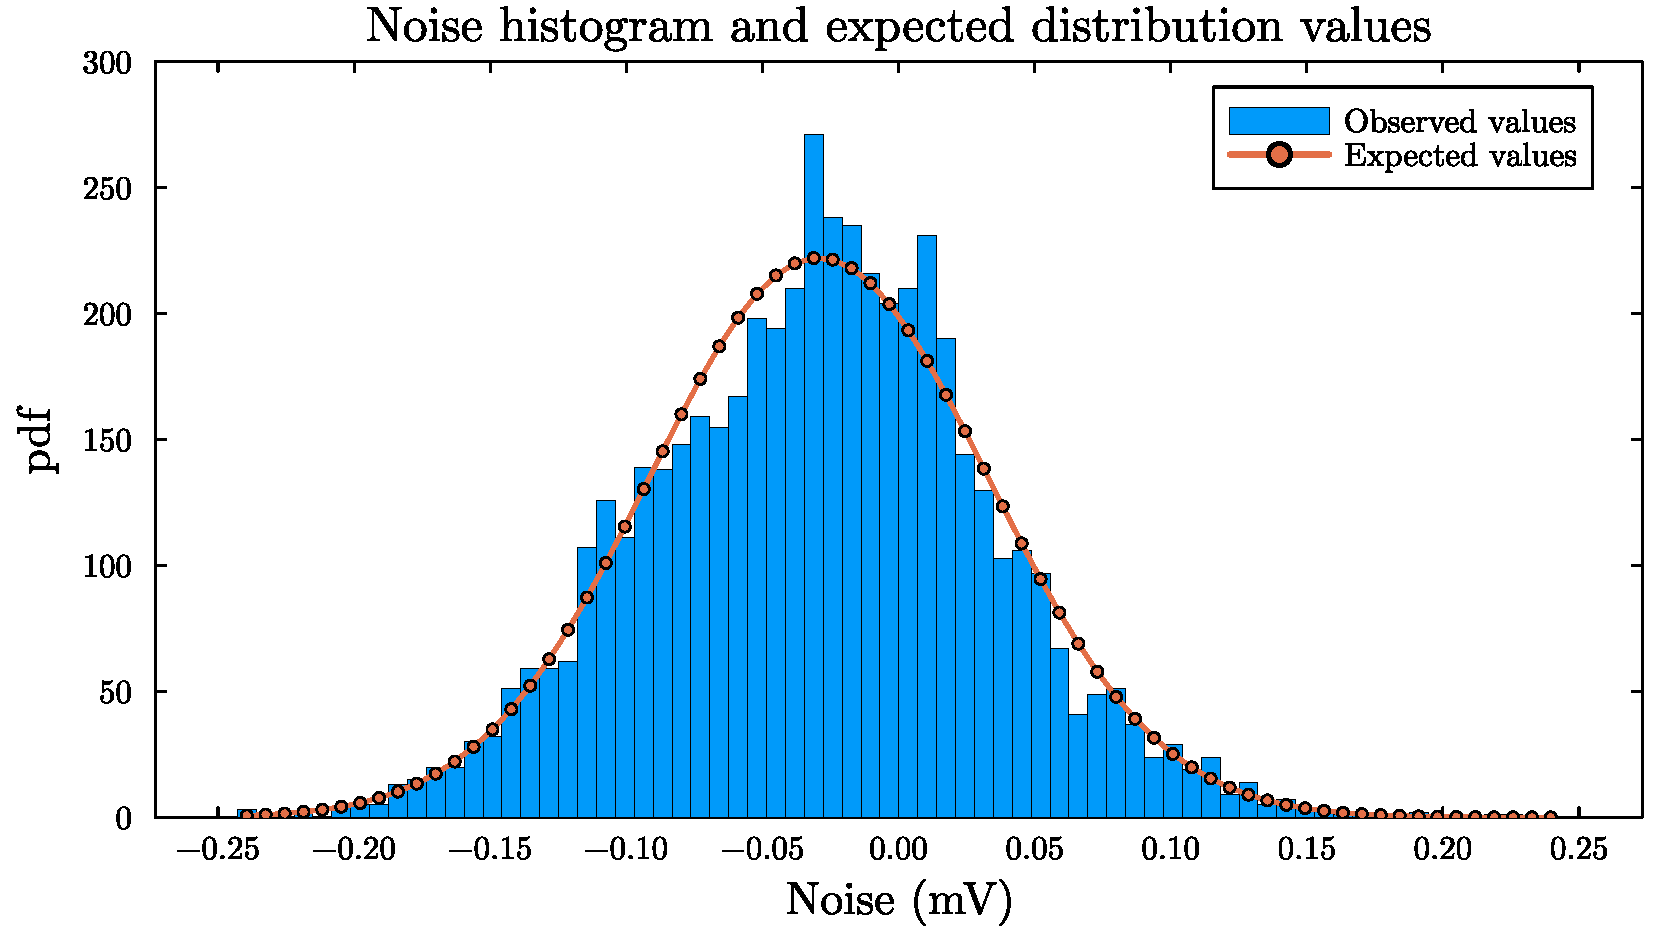
\includegraphics[width=0.9\textwidth]{Noise_hist_and_Normal_distr_expected_v.pdf}
    \caption{Histogram of the noise in overlay with the expected values given by the Gaussian distribution.}
    \label{plot:Hist_Gauss}
\end{figure}

\par Evaluating the chi squared gives us a result of $\chi^2 = 149.77$, 
with $d=70-3=67$ degrees of freedom. We can now obtain the reduced 
chi squared $\tilde{\chi}^2 = \chi^2 / d = 2.2354$. In this case, 
the probability to obtain a  $\chi^2$ ... is less than $0.05\%$, 
hence the distridution does not represent at all the collected data.
The Table (\ref{tab:summary_table}) 
sums up all the statistical data collected in this section.

\begin{table}[h]
    \centering
    \begin{tabular}{|c|c|}
        \hline
        Quantity & Value \\
        \hline
        Mean ($\mu$) & $-0.02925 \, mV$ \\
        \hline
        Standard error ($\sigma$) & $0.06231 mV$ \\
        \hline
        Degrees of freedom ($d$) & $67$ \\
        \hline
        Chi squared ($\chi^2$) & $149.77$ \\
        \hline
        Reduced chi squared ($\tilde{\chi}^2$) & $2.2354$ \\
        \hline
    \end{tabular}
    \caption{Summary table for the statistical quantities}
    \label{tab:summary_table}
\end{table}




\end{document}